\addcontentsline{toc}{section}{APPENDIX}

% Set footnotes to use letters
\renewcommand{\thefootnote}{\alph{footnote}}

\begin{landscape}

\begin{table}[!ht]
    \centering
    \begin{tabular}{|l|l|l|l|l|}
    \hline
        ~ & ~ & Model & ~ & ~ \\ \hline
        Field & Description & Thrombolysis use & Clinical outcome & Acute stroke pathway \\ \hline
        Stroke team & Stroke team attended (hospital identifier & y & y & y \\ \hline
        Age & Age (as midpoint of 5 year age bands) & y & y & y \\ \hline
        Sex & Sex of patient & ~ & ~ & y \\ \hline
        Atrial fibrillation diagnosis & Either on arrival or diagnosed during admission & ~ & y & y \\ \hline
        Use of atrial fibrillation anticoagulants & Use of prior anticoagulant for atrial fibrillation & y & ~ & y \\ \hline
        Precise onset known & If known whether it was known precisely or a best estimate & y & y & y \\ \hline
        Onset during sleep & Did stroke occur in sleep? & y & ~ & y \\ \hline
        Onset-to-arrival time & Time from onset of stroke to arrival at hospital (minutes) & y & y* & y \\ \hline
        Arrival-to-scan time & Time from arrival at hospital to scan (minutes) & y & y* & y \\ \hline
        Scan-to-thrombolysis time & Time from scan to treatment with thrombolysis (minutes) & T & y* & y \\ \hline
        Prior disability level & Estimated mRS score prior to stroke & y & y & y \\ \hline
        Stroke type & Infarction/haemorrhage & y & ~ & y \\ \hline
        Stroke severity & National Institutes of Health Stroke Scale score on arrival & y & y & y \\ \hline
        Disability on discharge & mRS (0-6) on discharge, includes death during admission & ~ & T & y \\ \hline
    \end{tabular}
\end{table}
\end{landscape}


\section{Method: Model to predict thrombolysis use}

\subsection{Data}

Data were retrieved for 78,396 emergency ischaemic stroke admissions that that arrived at an acute stroke team in England and Wales by ambulance after their stroke onset, and had their scan within 255 minutes of stroke onset, obtained from the Sentinel Stroke National Audit Programme (SSNAP) for six years, 2016–2021. SSNAP prospectively collects clinical data from 100\% of acute hospitals in England and Wales, with case ascertainment estimated at $>$90\% when compared with administrative coding data. The data excludes patients on anticoagulants (representing 12.9\% of the population) as information required to make a treatment decision may not be fully captured by the dataset (such as time anticoagulant medication last taken). The data includes 111 acute stroke teams (each with at least 250 stroke admissions  and which delivered thrombolysis to at least 10 patients in the study period). Data fields were provided for the hyper-acute phase of the stroke pathway, up to and including our target feature: disability on inpatient discharge. Disability is recorded in the SSNAP dataset using the modified Rankin Scale (mRS).


\subsection{Feature selection}

The full dataset contained 57 features that described patient characteristics, acute stroke pathway timings, use/time to thrombolysis, and the attended hospital. We were informed by clinical discussions and modelling to identify the features to include in the model, with the motivation to create an explainable model with fewer features that still captured the majority of the accuracy. We trained XGBoost thrombolysis outcome models on stratified 5-fold cross-validation data, sequentially selecting features to be included in the model as the single best feature to improve performance in terms of the area under the receiver operating characteristic (ROC AUC) curve. In 5-fold cross validation the data is split into 5 different 80:20 train/test splits with each patient being in one, and only one, test set. When included, the hospital attended and weekday feature were included as a one-hot encoded feature.

Code and full results for feature selection may be found at \url{https://github.com/samuel-book/feature_selection_thrombolysis_outcome_ml_paper}

\subsection{Machine learning model: Thrombolysis outcome}

In order to train a model to predict outcome from thrombolysis alone, we excluded the 2,747 patients who had received thrombectomy when training the outcome model. For the 75,649 patients that did not receive thrombectomy, we trained a multiclass classification XGBoost model (using stratified 5-fold cross-validation) to predict the mRS score at discharge from the other feature values (that describe the patients characteristics, their acute stroke pathway timings, use/time to thrombolysis, and the attended hospital). The resulting model prediction was a probability distribution across the seven mRS levels. We used stratified 5-fold cross-validation to test the accuracy of the model, for feature selection, and to test reproducibility of patterns detected. The results from the model fitted on the first k-fold split were used to investigate the relationships between feature values and their contribution to the prediction.

Code, and full results, for the machine learning work may be found at \url{https://github.com/samuel-book/thrombolysis_outcome_ml_paper}

\subsection{Model accuracy}

Model accuracy (using stratified 5-fold cross-validation) is reported as: percent correct, percent correct within one mRS category, sensitivity and specificity, ROC AUC, and confusion matrix. We used the multiclass method \textit{one vs rest} %\cite{fawcett_introduction_2006, hand_simple_2001} for computing the ROC AUC from the sklearn python package \cite{scikit-learn} which gives a measure of how well the model can identify the class from the other classes, on a class by class basis.

\subsection{SHapley Additive exPlanation (SHAP) values}

We sought to make our models explainable using SHAP values \cite{lundberg_unified_2017}. SHAP provides a measure of the contribution of each feature value to the final predicted likelihood of each of the seven levels of disability (mRS 0 to mRS 6) at discharge for that individual. SHAP values provided the influence of each feature as the change in log-odds of having a certain level of disability at discharge (SHAP values expressed as log-odds are additive; the final model log-odds prediction for an individual is the sum of all its feature SHAP values and the models baseline SHAP value, which is common across all individual predictions). A positive SHAP value represents that the corresponding feature value increases the likelihood for that individual to have that mRS level at discharge, and a negative SHAP value represents that the feature value reduces the likelihood for that patient to have that mRS level at discharge. SHAP values can be assessed \textit{locally} at patient level, and \textit{globally} at patient cohort level to understand general patterns of how discharge outcomes differ by each of the patient, pathway, and hospital characteristics. We also illustrated our model with \textit{prototype} patients which vary patient characteristics in a controlled way.

\subsection{Counterfactual treatment: Predicting if a patient would be likely to have a better outcome with or without thrombolysis}

We used the first k-fold \textit{thrombolysis outcome} model to calculate the counterfactual outcome for each treatment option (with and without thrombolysis) for the 15,680 patients in the first k-fold test set. We represented patients as receiving thrombolysis by setting the feature \textit{onset to thrombolysis time} to the sum of the recorded pathway durations for the patient (\textit{onset to arrival} and \textit{arrival to scan}) and added on the median \textit{scan to thrombolysis time} of their attended hospital. The median \textit{onset to thrombolysis time} for the 15,680 patients is 162 minutes (range 27 to 316 minutes). We represented patients as not receiving thrombolysis by setting the feature \textit{onset to treatment time} to 9,999 minutes. We translated the resulting two predicted probability distributions of disability at discharge (with and without thrombolysis) into a binary feature to represent whether the patient was predicted to have a better outcome receiving thrombolysis. We used a conservative definition to determine whether a patient has a better outcome with treatment from the two probability distributions, where both of these criteria must be met: 

\begin{enumerate}
    \item A reduction in probability-weighted mRS (a measure of the mid-point location of disability; it is the sum of each mRS outcome multiplied by the probability of that outcome occurring).
    \item A reduction in the likelihood of a very bad outcome (mRS 5-6, complete dependency or death).
\end{enumerate}

\subsection{Patient characteristics that contribute to a mismatch between actual thrombolysis use and predicted best outcome}

We analysed the distribution of feature values for the two patient cohorts that had a mismatch between the observed use of thrombolysis and a decison based on the machine learning model:

\begin{enumerate}
    \item Patients predicted by the \textit{thrombolysis outcome} model to have a better outcome with thrombolysis, but did not receive thrombolysis (1,842 patients) 
    
    \item Patients predicted by the \textit{thrombolysis outcome} to have a worse outcome with thrombolysis (an increase in either probability-weighted mRS or the probability of being mRS 5-6), but received thrombolysis (4,297 patients)
\end{enumerate}


\subsection{Hospital trade-off between maximising benefit from thrombolysis and minimising risk of harm from thrombolysis}

We trained an XGBoost \textit{thrombolysis decision} model on the first k-fold data split, to predict the likelihood of a patient receiving thrombolysis, using methods previously described \cite{pearn_what_2023}. We used this \textit{thrombolysis decision} model to predict the thrombolysis decision of each of the 15,680 patients in the first k-fold test set at each of the 111 stroke teams (by setting their feature \textit{stroke team} value to each of the stroke teams in turn). We used the \textit{thrombolysis outcome} model to predict the two mRS distributions at discharge (with and without treatment) for each of the 15,680 patients, and translated this into a binary feature to represent whether the patient was predicted to have a better outcome receiving thrombolysis. To remove the affect that hospital attended has on patient outcome at discharge, for each of the 15,680 patients in the first k-fold test set, we predicted outcomes at a hospital with the most neutral contribution to outcomes. To compare maximising benefit from thrombolysis and avoiding potential harm from thrombolysis we defined measures for \textit{sensitivity} and \textit{specificity} of treatment. \textit{Sensitivity} was calculated as the proportion of patients who were predicted to benefit from thrombolysis (from the \textit{thrombolysis outcome} model) who were predicted to receive thrombolysis at each team (from the \textit{thrombolysis decision} model). \textit{Specificity} was calculated as the proportion of patients who were predicted not to benefit from thrombolysis (from the \textit{thrombolysis outcome} model) who were not predicted to receive thrombolysis at each team (from the \textit{thrombolysis decision} model). A low \textit{sensitivity} would indicate a higher likelihood of not treating people who would benefit from thrombolysis, and a low \textit{specificity} would indicate a higher likelihood of treating people who would not benefit from thrombolysis.


\section{Method: Model to predict patient clinical outcome}

\section{Methods}

Note: further details of methods may be found in the online appendix. 

%%%%%%%%%%%%%%%%%%%%%%%%%%%%%%%%%%%%%%%%%%%%%%%%%%%%%%%%%%%%%%%%%%%%%%%%

\subsection{Data}

Data were retrieved for 246,676 emergency stroke admissions to acute stroke teams in England and Wales for the years 2016 - 2018, obtained from the Sentinel Stroke National Audit Programme (SSNAP). Data fields were provided for the hyper-acute phase of the stroke pathway, up to and including our target feature: \emph{receive thrombolysis}. Of these patients, 88,928 arrived within 4 hours of known stroke onset, and were used in this modelling study. The data included 132 acute stroke hospitals.

%%%%%%%%%%%%%%%%%%%%%%%%%%%%%%%%%%%%%%%%%%%%%%%%%%%%%%%%%%%%%%%%%%%%%%%%

\subsection{Machine learning models (to predict thrombolysis use)}

We used XGBoost \cite{chen_xgboost_2016} to predict the probability of use of thrombolysis for each patient from their other feature values.

%%%%%%%%%%%%%%%%%%%%%%%%%%%%%%%%%%%%%%%%%%%%%%%%%%%%%%%%%%%%%%%%%%%%%%%%

\subsubsection{Feature selection}

In order to simplify the model (for enhanced explainability) we selected those features most predictive of thrombolysis use. Features were selected by forward-feature selection, identifying one feature at a time that led to the greatest improvement in accuracy as measured by Receiver Operating Characteristic (ROC) Area Under Curve (AUC). We repeated this process to identify the top 25 features, and used these results to identify the number of features to include in our machine learning models.

%%%%%%%%%%%%%%%%%%%%%%%%%%%%%%%%%%%%%%%%%%%%%%%%%%%%%%%%%%%%%%%%%%%%%%%%

\subsubsection{Model accuracy}

Model accuracy, ROC AUC, sensitivity and specificity were measured using stratified 5-fold cross validation. Predicted thrombolysis rate was compared with actual thrombolysis use at hospital-level.

%%%%%%%%%%%%%%%%%%%%%%%%%%%%%%%%%%%%%%%%%%%%%%%%%%%%%%%%%%%%%%%%%%%%%%%%

\subsubsection{Machine learning models}

For the different analysis included in this paper, we trained three XGBoost models:
\begin{enumerate}
    \item \emph{K-fold} model: A 5-fold train-test cross validation used to test the accuracy of the model, and to test reproducibility of SHAP values.
       
    \item \emph{All data} model: A single model trained on all patients, used to investigate the relationship between feature values and predictions.
    
    \item \emph{10k holdout} model: A model trained on all data apart from a 10k hold-out set. This model is used to mimic a 10k cohort of patients that attends all hospitals (by changing the hospital encoding) to further investigate variation in thrombolysis decision-making between hospitals.
\end{enumerate}

%%%%%%%%%%%%%%%%%%%%%%%%%%%%%%%%%%%%%%%%%%%%%%%%%%%%%%%%%%%%%%%%%%%%%%%%
\subsection{SHapley Additive exPlanation (SHAP) values}

We sought to make our models explainable using SHAP values (calculated using the SHAP library \cite{lundberg_unified_2017}). SHAP provides a measure of the contribution of each feature value to the final predicted probability of receiving thrombolysis for that individual. The SHAP values for each feature are comprised of the feature’s main effect (the effect of that feature in isolation) and all of the pairwise interaction effects with each of the other features. SHAP values provide the influence of each feature as the change in log-odds of receiving thrombolysis (SHAP values expressed as log-odds are additive).

%%%%%%%%%%%%%%%%%%%%%%%%%%%%%%%%%%%%%%%%%%%%%%%%%%%%%%%%%%%%%%%%%%%%%%%%
\subsection{The relationship between feature values and the odds of receiving thrombolysis}

For each feature, we examined the relationship between feature values and their corresponding SHAP values (we used values from the \emph{all data} model).

%%%%%%%%%%%%%%%%%%%%%%%%%%%%%%%%%%%%%%%%%%%%%%%%%%%%%%%%%%%%%%%%%%%%%%%%
\subsection{Investigating how the identity of a hospital influences thrombolysis rate}

For each hospital we compared the mean SHAP main effect value for the hospital attended (using values from the \emph{all data} model) with the hospitals observed thrombolysis use.

To reveal the variation in thrombolysis rate due to hospital, rather than patient mix, we also compared the mean hospital attended SHAP main effect value for the identical 10k patient cohort attending each hospital, with the hospitals' predicted thrombolysis use for this 10k patient cohort (we used values from the \emph{10k holdout} model).

%%%%%%%%%%%%%%%%%%%%%%%%%%%%%%%%%%%%%%%%%%%%%%%%%%%%%%%%%%%%%%%%%%%%%%%%

\subsection{Investigating how patient populations and hospital identity and processes influences thrombolysis rate}

The 10 features in the model can be classified into two subsets: 1) `patient descriptive features' (features that describe the patients characteristics), and 2) `hospital descriptive features' (features that describe the hospital’s identity or processes). To analyse the influence that each subset of features has on the thrombolysis rate, using values from the \emph{all data} model, we calculated the `subset SHAP value' for each feature, which only includes the components of its SHAP value that contain effects from the features in the same subset. This is expressed as the sum of the main effect and the interaction effects with the other features in the same subset. Multiple regression models were then fitted to the mean subset SHAP values.

%%%%%%%%%%%%%%%%%%%%%%%%%%%%%%%%%%%%%%%%%%%%%%%%%%%%%%%%%%%%%%%%%%%%%%%%

\subsection{Variation in hospital thrombolysis use for patient subgroups}

Informed by the SHAP values, we analysed the observed and predicted use of thrombolysis in eleven subgroups of patients: one subgroup for `ideally' thrombolysable patients, nine `sub-optimal' thrombolysable patient subgroups (one subgroup per feature), and one subgroup with two sub-optimal features. The eleven patient subgroups were defined as:

\begin{enumerate}
  \item An \emph{`ideally'} thrombolysable patient:
  \begin{itemize}
    \setlength\itemsep{-2mm}
    \item Stroke caused by infarction
    \item Arrival-to-scan time $<$30 minutes
    \item NIHSS in range 10-25
    \item Precise stroke onset time known
    \item No pre-stroke disability (modified Rankin Scale, mRS, 0)
    \item Not taking atrial fibrillation anticoagulants
    \item Onset-to-arrival time $<$90 minutes
    \item Age $<$80 years old
    \item Onset not during sleep
  \end{itemize}
  \item Haemorrhagic stroke
  \item Arrival-to-scan time 60-90 minutes
  \item NIHSS $<$5
  \item Estimated stroke onset time
  \item Existing pre-stroke disability (mRS $>$2)
  \item Using atrial fibrillation anticoagulants
  \item Onset-to-arrival time 150-180 minutes
  \item Age 80+ years old
  \item Onset during sleep
  \item NIHSS $<$ 5 \emph{and} with estimated stroke onset time
\end{enumerate}

The observed thrombolysis use for each subgroup at each hospital was taken from the SSNAP dataset. In order to further reveal the variation in thrombolysis use that was due to hospital decision-making we predicted thrombolysis use for the same patient subgroups at each hospital by using the \emph{10k holdout} model.

%%%%%%%%%%%%%%%%%%%%%%%%%%%%%%%%%%%%%%%%%%%%%%%%%%%%%%%%%%%%%%%%%%%%%%%%





\section{Method: Model to simulate the acute stroke pathway}

\subsection{Overview}

\begin{figure}
    \centering
    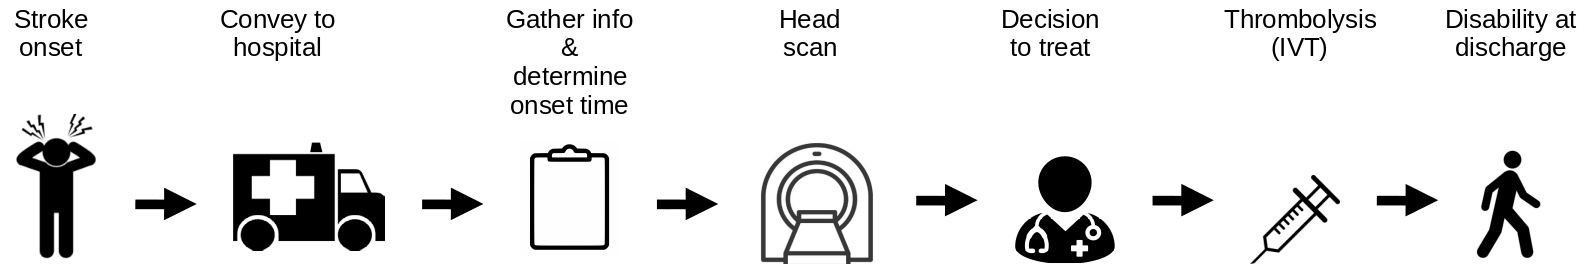
\includegraphics[width=1.0\linewidth]{images/flow}
    \caption{An overview of the process steps included in the modelling.}
    \label{fig:flow}
\end{figure}

Figure \ref{fig:flow} shows an overview of the process steps included in the modelling. Process flow was modelled by sampling from distributions of historic flow for each stroke team. Decision-making (choice of thrombolysis) was modelled with machine learning, learning which patients would likely be given thrombolysis at each stroke team. Outcomes were predicted using either mathematical models based on clinical trials (for the full pathway model), or clinical outcome machine learning models (for the more detailed analysis of differences in thrombolysis decision-making between teams).

\subsection{Data}

Data was used for all emergency stroke admissions to England and Wales for the 5 years 2017-2021, extracted from the national stroke registry for England, Wales and Northern Ireland, the Sentinel Stroke National Audit Programme (SSNAP). The registry contains all consecutive patients admitted to 100\% of acutely-admitting hospitals with a case ascertainment of over 90\% when compared to administrative data (Hospital Episode Statistics). Data was retrieved for teams with at least 250 admissions over the 5 years. The total number of patients was 302,715, of whom 114,625 (38\%) arrived within 4 hours of known stroke onset. Of those arriving within 4 hours of known stroke onset 103,244 (90\%) arrived by ambulance.

The following data fields from SSNAP were used in the modelling:

\begin{itemize}

    \item \textit{Stroke team}: Stroke team attended (hospital identifier).

    \item \textit{Age}: As midpoint of 5 year age bands.

    \item \textit{Sex}: Sex of patient (male/female)

    \item \textit{Diagnosis of atrial fibrillation}: Did the patient have a diagnosis of atrial fibrillation, either made prior to admission, or during admission?

    \item \textit{Use of anticoagulants}: Use of prior anticoagulant for atrial fibrillation.

    \item \textit{Onset known}: Whether onset was known, and if known whether it was considered to be known precisely or was a best estimate.

    \item \textit{Onset during sleep}: Did stroke occur in sleep? (1 = Yes, 0 = No).

    \item \textit{Onset-to-arrival time}: Time from onset of stroke to arrival at hospital (minutes), when known.

    \item \textit{Prior disability level}: Estimated modified Rankin Scale, mRS, prior to stroke.

    \item \textit{Stroke type}: Infarction/haemorrhage.

    \item \textit{Stroke severity}: National Institutes of Health Stroke Scale (NIHSS) score on arrival.

    \item \textit{Arrival-to-scan time}: Time from arrival at hospital to scan (minutes), when known.

    \item \textit{Scan-to-thrombolysis time}: Time from arrival at hospital to scan to treatment with thrombolysis  (minutes), when given.

    \item \textit{Disability on discharge}: mRS (0-6) on discharge, includes death (mRS 6) during admission.
    
\end{itemize}


\subsection{Thrombolysis decision model}

The thrombolysis decision model has been described in more detail previously \cite{pearn_what_2023}. Feature selection was used to identify 10 key features that were most predictive of whether thrombolysis was used in any given stroke team. The model uses XGBoost \cite{chen_xgboost_2016} for predictions, and SHAP \cite{lundberg_unified_2017} for local (patient-level) and global (model/population-level) explainability. SHAP values show the contribution of each feature value to the final model predictions.

The thrombolysis decision model was applied only to patients arriving within 4 hours of known stroke onset (stroke onset was known precisely or was a best estimate). The 10 features used for predicting thrombolysis use were: Stroke team; Age; Precisely known onset time; Onset during sleep; Onset-to-arrival time; Arrival-to-scan time; Stroke type; Stroke severity; Prior disability level; Use of anticoagulants.

%Code, with demonstration, is available \cite{allen_samuel_code_2024}.

\subsubsection{Prototype patients}

To help compare decision-making and outcomes across stroke teams we exemplified differences using \textit{prototype patients}. These prototype patients captured a range of features known to affect decisions to treat, and to affect outcomes, and included an \textit{ideal} candidate for thrombolysis. The prototype patients used were:

\begin{enumerate}
    \item \textit{Ideal}: Onset-to-arrival = 90 minutes; arrival-to-scan = 15 minutes; onset-to-thrombolysis = 120 minutes; stroke severity (NIHSS) = 15; pre-stroke disability (mRS) = 0; age = 72.5; precisely known onset; onset not during sleep; stroke type = infarction; patient has no atrial fibrillation and is not receiving anticoagulants for atrial fibrillation.

    \item \textit{Late arrival}: As \textit{ideal} but onset-to-arrival = 225 minutes and onset-to-thrombolysis (when given) = 255 minutes.

    \item \textit{Mild}: As \textit{ideal} but stroke severity = 3.

    \item \textit{Prior disability}: As \textit{ideal} but pre-stroke disability = 3

    \item \textit{Imprecise}: As \textit{ideal} but stroke onset time estimated.

    \item \textit{Age}: As \textit{ideal} but age = 87.5.

    \item Combinations of the above.
\end{enumerate}

\subsubsection{Benchmark stroke teams and benchmark decisions}

SHAP isolates the contributes of features to model predictions. As one feature is the stroke team, the stroke team SHAP shows the influence of attending that stroke team on the likelihood of a patient receiving thrombolysis. Averaging stroke team SHAP values for all patients attending a given hospital provided a measure of the overall willingness of that stroke team to use thrombolysis (or how much that stroke team affected the odds of a patient receiving thrombolysis in the model). We took the stroke teams with the 25 highest stroke team SHAP values as \textit{benchmark stroke teams}. For any given patient, predictions can be made about whether each of the stroke teams would, or would not, give that patient thrombolysis. We took a majority vote of those 25 decisions as a \textit{benchmark decision} for that patient.

\subsection{Stroke outcome machine learning model}

The machine learning model predicting disability/death at discharge (mRS) is described in more detail in a companion paper \cite{pearn_are_2024}. Briefly, we used XGBoost \cite{chen_xgboost_2016} to predict outcome (mRS level) based on the following features:

\begin{enumerate}
    \item \textit{Prior disability level}: Disability level (mRS) before stroke
    \item \textit{Stroke severity}: Stroke severity (NIHSS) on arrival
    \item \textit{Stroke team}: Attended hospital
    \item \textit{Age}: Age (as middle of 5 year age bands)
    \item \textit{Onset to thrombolysis time}: Time from onset to receiving thrombolysis (minutes). Set to 9999 if did not receive thrombolysis.
    \item \textit{Any afib diagnosis}: Patient has a diagnosis of atrial fibrillation (either on arrival or new)
    \item \textit{Precise onset known}: Onset time recorded is precise time (not a best estimate)
\end{enumerate}

\subsection{Mild stroke}

We used the machine learning and decision models to specifically investigate the expected benefit or harm from mild stroke (NIHSS 0-4) in three groups: 1) All admissions within 4 hours of stroke onset, 2) Patients who had received thrombolysis, 3) Patients where the \textit{benchmark decision} would be to give thrombolysis.

\subsection{Lifetime economic model}

Data about further admissions and mortality was provided for acute stroke patients discharged between 2013 and 2014 from a large English service.  This was combined with data from UK life tables to create a set of parametric equations in a model that use age, sex, and modified Rankin Scores to predict the life-time risk of mortality and secondary care resource utilisation including Emergency Department attendances, non-elective admissions, and elective admissions. A cohort of 1,509 (male 51\%; mean age 74) stroke patients had median follow-up of seven years and represented 7,111 post-discharge patient years.  A logistic model estimated mortality within twelve months of discharge and a Gompertz model was used over the remainder of the lifetime. Hospital attendances were modelled using a Weibull distribution. Non-elective and elective bed days were both modelled using a log-logistic distribution. Assumed utiltites by mRS at discharge were based on values reported by Dijkland \textit{et al}. %\cite{dijkland_utility-weighted_2018}. The lifetime economic model is described in detail by McMeekin \textit{et al}. \cite{mcmeekin_lifetime_2024}, and a full code for the economic model is available \cite{laws_stroke-optimiststreamlit_lifetime_stroke_2024}.

\subsection{Pathway model}

The pathway model has been described in more detail previously \cite{allen_use_2022}, though has been extended here to model changes in the pre-hospital pathway (ambulance response). Briefly, we model processes, including variation, using a Monte Carlo simulation model of the clinical pathway. This samples onset-to-arrival times, process times, determination of stroke onset time, and decision to thrombolyse from distributions based on historic data for each stroke team. The model predicts thrombolysis use and times for a year's admission to each stroke team (100 replicates are run, simulating 100 years admissions). Clinical outcome is predicted as the number of \textit{good outcomes} (mRS 0-1) per 1,000 admissions using a previously described mathematical model \cite{allen_estimation_2020}.

The pathway model may be used to examine a range of possible changes to improve use and speed of thrombolysis:

\begin{enumerate}

    \item \textit{Base}: Uses the hospitals’ recorded pathway statistics.

    \item \textit{Speed}: Sets 95\% of patients having a scan within 4 hours of arrival, and all patients have 15 minutes arrival-to-scan time and 15 minutes scan-to-needle time.

    \item \textit{Ambo}: Subtracts 15 minutes from the current ambulance call to arrival-at-hospital times.

    \item  \textit{Onset-known}: Sets the proportion of patients with a known stroke onset time to the national upper quartile (79.6\%) if currently less than the national upper quartile.

    \item \textit{Benchmark}: The benchmark thrombolysis rate takes the likelihood to give thrombolysis for patients scanned within 4 hours of onset from the majority vote of the 25 benchmark hospitals (see above).

    \item Combinations of the above.
    
\end{enumerate}

Code, with demonstration, is available at \url{https://github.com/samuel-book/samuel_2_demo}.
















\section{Descriptive statistics}
\label{sec:stats}

Tables \ref{tab:hospital_stats_1} to \ref{tab:hospital_stats_3} show descriptive statistics for patients (2016-2021) across all stroke teams for (1) all patients, patients arriving within 4 hours of known stroke onset, and patients arriving by ambulance within 4 hours of known stroke onset.

\begin{minipage}{1\textwidth}
\small
\renewcommand{\arraystretch}{1.3}
\begin{longtable}{p{7cm} p{1cm} p{0.8cm} p{0.8cm} p{0.8cm} p{0.8cm} p{0.8cm} p{0.8cm} p{0.8cm} p{0.8cm}}
\caption{Descriptive statistics for all patients (n = 360,381) arriving at each stroke team. The table shows summary statistics across all stroke teams capturing each feature.}\\
\toprule
\endhead
Statistic & Stroke teams & mean & Std Dev & min & 25\% & 50\% & 75\% & max\tabularnewline
\midrule
Yearly admissions & 119 & 509 & 208 & 95 & 372 & 489 & 627 & 1183\tabularnewline
Age (mean) & 119 & 74 & 2 & 65 & 73 & 75 & 76 & 78\tabularnewline
Proportion aged 80+ & 119 & 0.40 & 0.06 & 0.20 & 0.36 & 0.40 & 0.44 & 0.51\tabularnewline
Proportion male & 119 & 0.53 & 0.02 & 0.47 & 0.51 & 0.53 & 0.55 & 0.60\tabularnewline
Prior disability (mRS, mean) & 119 & 1.02 & 0.25 & 0.29 & 0.87 & 1.03 & 1.21 & 1.60\tabularnewline
Proportion prior disability (mRS) 0-2 & 119 & 0.81 & 0.05 & 0.67 & 0.78 & 0.81 & 0.84 & 0.97\tabularnewline
Proportion ischaemic stroke & 119 & 0.88 & 0.02 & 0.83 & 0.86 & 0.88 & 0.89 & 0.93\tabularnewline
Stroke severity (NIHSS, mean) & 119 & 7.0 & 1.0 & 4.6 & 6.3 & 7.2 & 7.8 & 9.1\tabularnewline
Proportion with known onset & 119 & 0.68 & 0.14 & 0.43 & 0.58 & 0.67 & 0.76 & 1.00\tabularnewline
Onset-to-arrival time (minutes, median) & 119 & 204 & 76 & 109 & 155 & 180 & 224 & 466\tabularnewline
Proportion arriving within 4 hours known onset & 119 & 0.38 & 0.06 & 0.19 & 0.34 & 0.38 & 0.43 & 0.51\tabularnewline
Proportion with precisely known onset & 119 & 0.33 & 0.11 & 0.01 & 0.28 & 0.34 & 0.39 & 0.63\tabularnewline
Proportion onset during sleep & 119 & 0.14 & 0.06 & 0.00 & 0.09 & 0.14 & 0.17 & 0.34\tabularnewline
Proportion arrive by ambulance & 119 & 0.78 & 0.07 & 0.47 & 0.76 & 0.79 & 0.82 & 0.92\tabularnewline
Call-to-ambulance arrival time (minutes, median) & 113 & 22 & 10 & 13 & 17 & 20 & 24 & 103\tabularnewline
Ambulance on scene time (median) & 113 & 31 & 3 & 20 & 28 & 31 & 33 & 41\tabularnewline
Ambulance conveyance time (minutes, median) & 113 & 18 & 5 & 10 & 15 & 17 & 21 & 37\tabularnewline
Arrival-to-scan time (minutes, median) & 119 & 53 & 21 & 13 & 39 & 51 & 63 & 129\tabularnewline
Proportion receiving thrombolysis & 119 & 0.115 & 0.034 & 0.021 & 0.092 & 0.110 & 0.136 & 0.245\tabularnewline
Scan-to-thrombolysis time (minutes, median) & 119 & 34 & 10 & 14 & 28 & 34 & 41 & 72\tabularnewline
Discharge disability (mRS, mean) & 119 & 2.641 & 0.352 & 1.361 & 2.413 & 2.699 & 2.900 & 3.320\tabularnewline
Proportion discharged mRS 0-2 & 119 & 0.524 & 0.095 & 0.293 & 0.454 & 0.522 & 0.594 & 0.799\tabularnewline
Proportion discharged mRS 5-6 & 119 & 0.195 & 0.037 & 0.095 & 0.170 & 0.198 & 0.218 & 0.287\tabularnewline
\bottomrule
\label{tab:hospital_stats_1}
\end{longtable}
\normalsize
\end{minipage}


\begin{minipage}{1\textwidth}
\small
\begin{longtable}{p{7cm} p{1cm} p{0.8cm} p{0.8cm} p{0.8cm} p{0.8cm} p{0.8cm} p{0.8cm} p{0.8cm} p{0.8cm}}
\caption{Descriptive statistics for patients (n = 138,946) arriving within 4 hours of known stroke onset at each stroke team. The table shows summary statistics across all stroke teams capturing each feature.}\\
\toprule
\endhead
Statistic & Stroke teams & mean & Std Dev & min & 25\% & 50\% & 75\% & max\tabularnewline
\midrule
Yearly admissions & 119 & 193 & 78 & 28 & 139 & 183 & 241 & 428\tabularnewline
Age (mean) & 119 & 75 & 2 & 66 & 73 & 75 & 76 & 79\tabularnewline
Proportion aged 80+ & 119 & 0.41 & 0.06 & 0.23 & 0.37 & 0.41 & 0.45 & 0.57\tabularnewline
Proportion male & 119 & 0.53 & 0.03 & 0.45 & 0.51 & 0.53 & 0.55 & 0.64\tabularnewline
Prior disability (mRS, mean) & 119 & 1.04 & 0.25 & 0.37 & 0.88 & 1.04 & 1.22 & 1.60\tabularnewline
Proportion prior disability (mRS) 0-2 & 119 & 0.80 & 0.06 & 0.66 & 0.77 & 0.81 & 0.83 & 0.95\tabularnewline
Proportion ischaemic stroke & 119 & 0.85 & 0.03 & 0.75 & 0.84 & 0.85 & 0.87 & 0.94\tabularnewline
Stroke severity (NIHSS, mean) & 119 & 8.9 & 1.1 & 6.4 & 8.2 & 9.0 & 9.7 & 11.4\tabularnewline
Proportion with known onset & 119 & 1.00 & 0.00 & 1.00 & 1.00 & 1.00 & 1.00 & 1.00\tabularnewline
Onset-to-arrival time (minutes, median) & 119 & 105 & 9 & 85 & 100 & 105 & 111 & 132\tabularnewline
Proportion arriving within 4 hours known onset & 119 & 1.00 & 0.00 & 1.00 & 1.00 & 1.00 & 1.00 & 1.00\tabularnewline
Proportion with precisely known onset & 119 & 0.62 & 0.17 & 0.02 & 0.54 & 0.66 & 0.75 & 0.91\tabularnewline
Proportion onset during sleep & 119 & 0.05 & 0.05 & 0.00 & 0.01 & 0.03 & 0.06 & 0.30\tabularnewline
Proportion arrive by ambulance & 119 & 0.89 & 0.07 & 0.54 & 0.87 & 0.91 & 0.93 & 0.98\tabularnewline
Call-to-ambulance arrival time (minutes, median) & 110 & 19 & 5 & 8 & 16 & 18 & 21 & 51\tabularnewline
Ambulance on scene time (median) & 110 & 28 & 4 & 20 & 26 & 28 & 31 & 46\tabularnewline
Ambulance conveyance time (minutes, median) & 110 & 17 & 4 & 9 & 14 & 16 & 20 & 28\tabularnewline
Arrival-to-scan time (minutes, median) & 119 & 27 & 11 & 4 & 21 & 28 & 34 & 100\tabularnewline
Proportion receiving thrombolysis & 119 & 0.293 & 0.070 & 0.111 & 0.250 & 0.282 & 0.333 & 0.534\tabularnewline
Scan-to-thrombolysis time (minutes, median) & 119 & 34 & 10 & 14 & 28 & 34 & 40 & 71\tabularnewline
Discharge disability (mRS, mean) & 119 & 2.803 & 0.353 & 1.507 & 2.609 & 2.837 & 3.039 & 3.663\tabularnewline
Proportion discharged mRS 0-2 & 119 & 0.494 & 0.094 & 0.209 & 0.424 & 0.495 & 0.554 & 0.771\tabularnewline
Proportion discharged mRS 5-6 & 119 & 0.236 & 0.045 & 0.138 & 0.208 & 0.231 & 0.256 & 0.420\tabularnewline
\bottomrule
\label{tab:hospital_stats_2}
\end{longtable}
\normalsize
\end{minipage}

\begin{minipage}{1\textwidth}
\small
\begin{longtable}{p{7cm} p{1cm} p{0.8cm} p{0.8cm} p{0.8cm} p{0.8cm} p{0.8cm} p{0.8cm} p{0.8cm} p{0.8cm}}
\caption{Descriptive statistics for patients (n = 125,557) arriving by ambulance within 4 hours of known stroke onset at each stroke team. The table shows summary statistics across all stroke teams capturing each feature.}\\
\toprule
\endhead
Statistic & Stroke teams & mean & Std Dev & min & 25\% & 50\% & 75\% & max\tabularnewline
\midrule
Yearly admissions & 119 & 173 & 74 & 15 & 125 & 163 & 227 & 400\tabularnewline
Age (mean) & 119 & 75 & 2 & 66 & 74 & 76 & 77 & 81\tabularnewline
Proportion aged 80+ & 119 & 0.43 & 0.06 & 0.24 & 0.39 & 0.43 & 0.47 & 0.62\tabularnewline
Proportion male & 119 & 0.52 & 0.03 & 0.45 & 0.51 & 0.52 & 0.54 & 0.60\tabularnewline
Prior disability (mRS, mean) & 119 & 1.10 & 0.25 & 0.46 & 0.94 & 1.09 & 1.26 & 1.66\tabularnewline
Proportion prior disability (mRS) 0-2 & 119 & 0.79 & 0.06 & 0.65 & 0.75 & 0.79 & 0.83 & 0.93\tabularnewline
Proportion ischaemic stroke & 119 & 0.85 & 0.03 & 0.75 & 0.83 & 0.85 & 0.87 & 0.94\tabularnewline
Stroke severity (NIHSS, mean) & 119 & 9.4 & 1.2 & 6.7 & 8.6 & 9.5 & 10.2 & 12.2\tabularnewline
Proportion with known onset & 119 & 1.00 & 0.00 & 1.00 & 1.00 & 1.00 & 1.00 & 1.00\tabularnewline
Onset-to-arrival time (minutes, median) & 119 & 106 & 10 & 84 & 99 & 105 & 112 & 151\tabularnewline
Proportion arriving within 4 hours known onset & 119 & 1.00 & 0.00 & 1.00 & 1.00 & 1.00 & 1.00 & 1.00\tabularnewline
Proportion with precisely known onset & 119 & 0.62 & 0.17 & 0.02 & 0.54 & 0.65 & 0.75 & 0.92\tabularnewline
Proportion onset during sleep & 119 & 0.05 & 0.05 & 0.00 & 0.01 & 0.03 & 0.06 & 0.33\tabularnewline
Proportion arrive by ambulance & 119 & 1.00 & 0.00 & 1.00 & 1.00 & 1.00 & 1.00 & 1.00\tabularnewline
Call-to-ambulance arrival time (minutes, median) & 110 & 19 & 5 & 8 & 16 & 18 & 21 & 51\tabularnewline
Ambulance on scene time (median) & 110 & 28 & 4 & 20 & 26 & 28 & 31 & 46\tabularnewline
Ambulance conveyance time (minutes, median) & 110 & 17 & 4 & 9 & 14 & 16 & 20 & 28\tabularnewline
Arrival-to-scan time (minutes, median) & 119 & 26 & 11 & 4 & 20 & 25 & 33 & 95\tabularnewline
Proportion receiving thrombolysis & 119 & 0.300 & 0.072 & 0.130 & 0.252 & 0.289 & 0.345 & 0.537\tabularnewline
Scan-to-thrombolysis time (minutes, median) & 119 & 34 & 10 & 13 & 27 & 33 & 40 & 73\tabularnewline
Discharge disability (mRS, mean) & 119 & 2.926 & 0.352 & 1.867 & 2.717 & 2.928 & 3.150 & 3.819\tabularnewline
Proportion discharged mRS 0-2 & 119 & 0.465 & 0.096 & 0.184 & 0.398 & 0.462 & 0.524 & 0.696\tabularnewline
Proportion discharged mRS 5-6 & 119 & 0.254 & 0.051 & 0.147 & 0.221 & 0.253 & 0.280 & 0.486\tabularnewline
\bottomrule
\label{tab:hospital_stats_3}
\end{longtable}
\normalsize
\end{minipage}

%%%%%%%%%%%%%%%%%%%%%%%%%%%%%%%%%%%%%%%%%%%%%%%%%%%%%%%%%%%%%%%%%%%%%%%%%%%%%%%%%%%
\section{Review of objectives set in original bid}
\label{sec:objectives_met}

The following outlines the key objectives set out in the original bid, and what has been delivered:

\subsection{Objective 1: Expansion of SAMueL-1 modelling}

\subsubsection*{Objective}

Expansion of previous (SAMueL-1) modelling to include: 1) outcome and adverse event prediction at patient-level, 2) inclusion of pre-hospital times in pathway model, 3) use of organisational factors (such as staffing) in predicting use of thrombolysis, and 4) piloting of a model that incorporates use of thrombectomy alongside thrombolysis.

\subsubsection*{Project outputs}

All objectives were achieved and reported:

\begin{itemize}
    \item Outcome models are reported and used in sections %\ref{sec:paper_3}, \ref{sec:paper_4}, and \ref{sec:paper_5}. Outcome and adverse event prediction at patient-level were predicted in the patient-level outcome model. We chose to use an all-cause beneficial/adverse outcome, rather than specific adverse events such as thrombolysis-induced haemorrhage. This was because we were primarily interested in net benefit or disbenefit from thrombolysis. Adverse outcomes associated with thrombolysis were taken as increased risk of severe death or disability (mRS 5-6). Outcome prediction was a very substantial part of this project, and included.
    \begin{itemize}
        \item Development of models that predict probability of outcome across all disability (mRS) levels, and separate models to predict being within any given disability threshold on discharge.
        \item The addition of Shapley values (SHA) to outcome predictions, allow us to show, and analyse the contribution of individual features (such as use/time of thrombolysis) to patient outcomes.
        \item A comparison of the observed effect of thrombolysis (from our analysis) with clinical trial meta0analysis of thrombolysis.
        \item A comparison of who receives thrombolysis with who will benefit from thrombolysis (from our outcome models).
    \end{itemize}
    \item Pre-hospital times (ambulance response and on-scene times) were included in the pathway model, and were used as a possible scenario for improvement (see section %\ref{sec:paper_5}).    
    \item We performed a multiple regression analysis on organisational factors from the SSNAP audit. We did not find any significant link to willingness to use thrombolysis (see %\ref{sec:other_outputs}).
    \item We performed a pilot model on the benefit from thrombectomy (and confirmed a beneficial effect that declines over time). The data set was small for this intervention and more work will be required to make this work suitable for publication (we have included pilot work in section %\ref{sec:other_outputs} (\textit{Other project outputs} as results should be considered indicative rather than at a level suitable for robust peer review.)       
\end{itemize}


%%%%%%%%%%%%%%%%%%%%%%%%%%%%%%%%%%%%%%%%%%%%%%%%%%%%%%%%%

\subsection{Objective 2: Incorporation of health economic outcomes}

\subsubsection*{Objective}

Incorporation of health economic outcomes (Quality Adjusted Life Years, QALYs): These will be adapted from other NIHR projects involving this team that have already developed health economic models for thrombolysis in acute ischaemic stroke.

This objective was achieved and reported:

\subsubsection*{Project outputs}

\begin{itemize}
    \item A health economics model for stroke has been coded by the SAMueL team and is available on GitHub (\url{https://github.com/stroke-optimist/stroke-lifetime} and available for installation on Python from PyPI (\url{https://pypi.org/project/stroke-lifetime/}).
    \item The effect of thrombolysis on, life expectancy, QALYs, NHS care costs, and cost per QALY are included in section \ref{sec:paper_5}.
\end{itemize}

%%%%%%%%%%%%%%%%%%%%%%%%%%%%%%%%%%%%%%%%%%%%%%%%%%%%%%%%%

\subsection{Objective 3: Promote acceptance of the modelling by increased transparency and explainability}

\subsubsection*{Objective}

Promote acceptance of the modelling by increased transparency and explainability: 1) make use of Shapley values to show the contribution of individual features to the prediction that the model is making, 2) improved methods for clustering of patients to clarify patterns of differences in clinical decision-making between hospitals and to allow identification of ‘similar hospitals’ (by patient population) for comparison, 3) investigation of bias in model (e.g. accuracy analysis by patient subgroups), 4) generation of dashboards and other interrogative methods.


\subsubsection*{Project outputs}

All objectives were achieved and reported, except we did not have the data to analyse model accuracy by key demographic groups (as we were concerned about possible identification of people by inclusion of ethnicity; though we have a plan for for for future work):

\begin{itemize}
    \item Shapley values have been used extensively to explore the relationship between patient features and model predictions (thrombolysis use, and outcomes). These have been performed at patient and population level. %See sections \ref{sec:paper_2}, \ref{sec:paper_3}, \ref{sec:paper_4}.
    \item We identified key characteristics of patients where stroke teams make different decisions and condensed these into prototype patients. This allowed us to identify stroke teams that were, for example, less likely to give thrombolysis to patients with mild stroke, pre-stroke disability or with imprecisely known stroke onset times. See sections %\ref{sec:paper_2} and \ref{sec:paper_5}.
    \item Shapely values help reveal 'bias' in the model by showing how patient features affect model predictions. We did not analyse accuracy by subgroup. In our final data request we did not include ethnicity as we had some concern about identification of patients in small minority groups. In future work we will ask for 2-3 ethnic groups and include others as 'other' and we will reduce the granularity of other data (such as month of attendance) to avoid possible identification. This will allow us to perform an analysis of thrombolysis use and outcomes, and model accuracy by ethnicity. We will also access decile of Index of Multiple Deprivation to perform similar analysis by this index.
    \item Our models have been made available as web app dashboard: \url{https://stroke-predictions.streamlit.app/}. At this stage we have not included patient-level outcome predictions due to a concern that it could be used for clinical decision-making. 
\end{itemize}



%%%%%%%%%%%%%%%%%%%%%%%%%%%%%%%%%%%%%%%%%%%%%%%%%%%%%%%%%

\subsection{Objective 4: Generation of synthetic data and artificial patient vignettes}

\subsubsection*{Objective}

Generation of synthetic data and artificial patient vignettes: 1) build on pilot work already performed for generating synthetic patient-level stroke data that may be shared freely and used for discussion of ’virtual’ patients, 2) automatic generation of artificial clinical vignettes from real or synthetic SSNAP data.

\subsubsection*{Project outputs}

These objectives were achieved, but in a slightly different way to planned:

\begin{itemize}
    \item We were able to make artificial patient data by crudely sampling key patient characteristics, but then allocating thrombolysis use and outcomes based on model predictions based on real patients. These data are made available in the project code demonstration GitHub repository: \url{https://stroke-predictions.streamlit.app/}.
    \item As we simplified models to as few patient features as necessary for good predictions we are able to describe patients succinctly. We also developed \textit{prototype patients} that could be used to compare outcomes (see section \ref{sec:paper_5}).    
\end{itemize}


%%%%%%%%%%%%%%%%%%%%%%%%%%%%%%%%%%%%%%%%%%%%%%%%%%%%%%%%%

\subsection{Objective 5: Co-production of project outputs with clinicians to promote acceptance and use for local quality improvement}

\subsubsection*{Original objective:}

Co-production of project outputs with clinicians to promote acceptance and use for local quality improvement: By using both information gathering (through interviews) and intervention refinement (in workshops) we will incrementally modify and improve the content and style of our intervention (SAMueL tool). Working with our Public and Patient Involvement (PPI) group we will also produce key public-facing output.

\subsubsection*{Amended objective}

With agreement of NIHR (through a \textit{Variation to Contract} agreement) the qualitative approach was altered to:

What should a machine-learning model based on SSNAP data look like, do, and deliver if it is to optimise improvement, and reduce unwarranted variation, in thrombolysis?

\begin{enumerate}
    \item To generate empirically and theoretically informed knowledge about how thrombolysis is currently delivered, centred on physicians’ views, understandings, and practices.
    \item To learn more about how stroke physicians’ and staff think and feel about or use SSNAP, and about the use of machine learning in improving clinical practice.
\end{enumerate}


\subsubsection*{Project outputs}

%All objectives of the revised objectives were met (section \ref{sec:paper_1}).

Using the NASS framework we identified three learning points which, if addressed, may facilitate further implementation of the technology. 

\begin{itemize}
    \item Given reservations expressed by some of our participants and healthcare professionals elsewhere about the underpinning SSNAP data it seems important to ensure that intended adopters are reassured about the integrity of modelling based on this data.
    \item Evidence from this research and elsewhere indicates that the ED physicians’ may have less confidence in the evidence base for, and safety of thrombolysis. It is therefore likely that more work will need to be done with the ED physician community to build trust in the SAMuel-2 technology: recruiting ED physicians as brokers/clinical champions may help to address this.
    \item Perceived lack of funding/resource and stroke workforce shortages may impede quality improvement and adoption of new technologies such as SAMueL-2.
\end{itemize}